\frame{
  \frametitle{The context}
\begin{center} 
Easy understanding with effective representation
 \end{center}
  \begin{figure}[H]
    \centering
    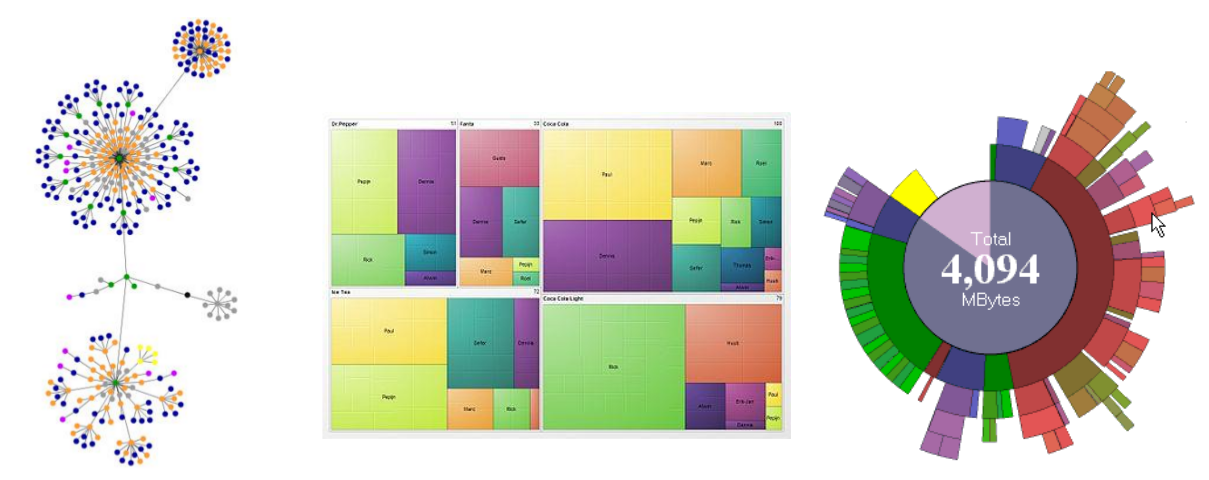
\includegraphics[scale=0.29]{../rapport/img/graphes_jolis.png}
  \end{figure}
  \pause
  \begin{alertblock}{}
  \centering
    Only available for few graphs
\end{alertblock}
\vspace{1cm}
} 

\frame{
  \frametitle{The context}
  \framesubtitle{Two different methods}
  \begin{figure}[H]
    \centering
    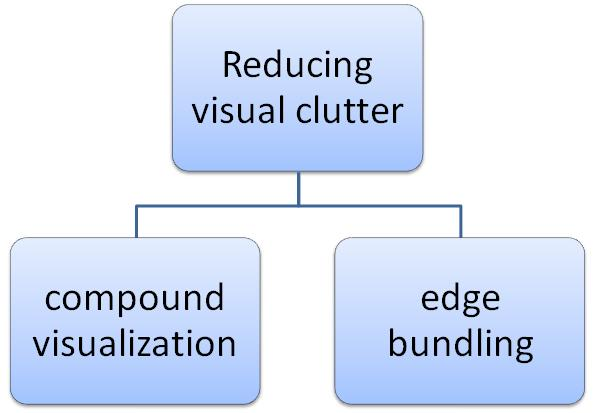
\includegraphics[scale=0.4]{../rapport/img/slide3.jpg}
  \end{figure}
 
\vspace{1cm}
} 

\frame{
  \frametitle{The context}
  \framesubtitle{Compound visualization}
  \begin{figure}[H]
    \centering
    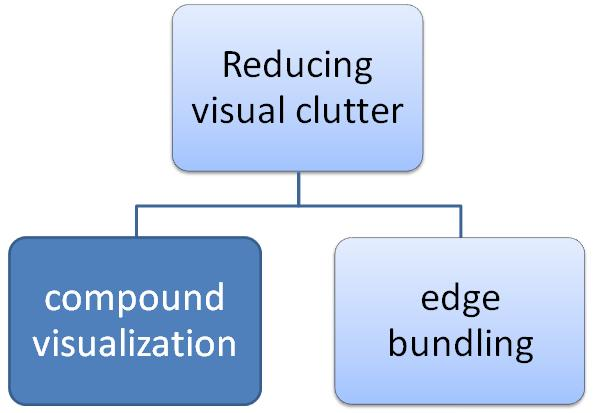
\includegraphics[scale=0.4]{../rapport/img/slide4.jpg}
  \end{figure}
 
\vspace{1cm}
} 

\frame{
  \frametitle{The context}
  \framesubtitle{Compound visualization}
  
  \begin{columns}[!ht]
    \begin{column}{4cm}
    \begin{block}{}   
     \begin{itemize}
     \item Nodes gathered into metanodes\\
     \item Inter-cluster edges merged into metaedges
     \end{itemize}
     \end{block}
    \end{column}
    \begin{column}{6cm}   
      \begin{figure}[H]
        \centering
        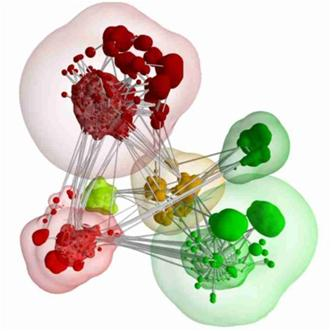
\includegraphics[scale=0.5]{../rapport/img/slide5.jpg}
      \end{figure}
    \end{column}
  \end{columns}
 \pause

  \begin{alertblock}{}
  \centering
    Impossibility for some nodes to move:
    node positions bring information
\end{alertblock}

\vspace{1cm}
} 

\frame{
  \frametitle{The context}
  \framesubtitle{Edge bundling}
  \begin{figure}[H]
    \centering
    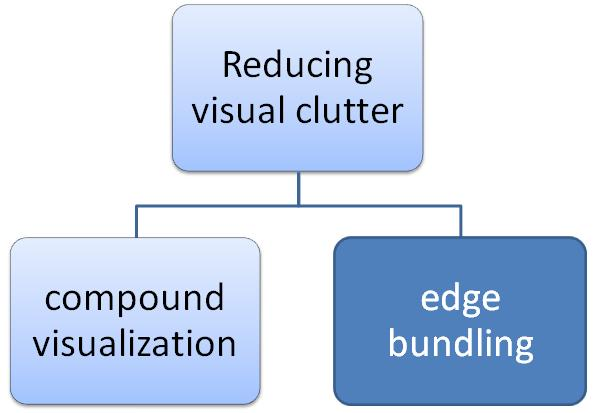
\includegraphics[scale=0.4]{../rapport/img/slide6.jpg}
  \end{figure}
 
\vspace{1cm}
} 

\frame{
  \frametitle{The context}
  \framesubtitle{Edge bundling}

\begin{alertblock}{}
  \centering
    Impossibility for some nodes to move:
    node positions bring information
\end{alertblock}
\pause
\begin{figure}[H]
        \centering
        
\includegraphics[scale=0.2]{../rapport/img/fleche.png}
      \end{figure}
\begin{center}
\begin{exampleblock}{}
\centering
Keep node position but edge aggregation
\end{exampleblock}
\end{center}                 
\pause 
 \begin{columns}[!ht]
\vspace{1cm}
    \begin{column}{6cm} 
    \begin{block}{}
    \centering
    Routes edges into bundles
    \end{block}
    \end{column}
    \begin{column}{6cm}   
      \begin{figure}[H]
        \centering
        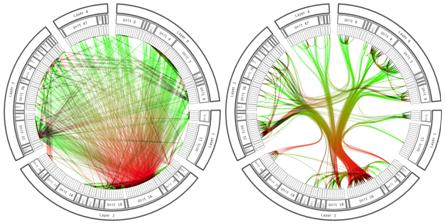
\includegraphics[scale=0.5]{../rapport/img/slide7_2.jpg}
      \end{figure}
    \end{column}
  \end{columns}

} 

\frame{
  \frametitle{The context}
  \framesubtitle{Problematic}

 \begin{columns}[!ht]
\vspace{1cm}
    \begin{column}{6cm} 
    \begin{block}{}
    \begin{itemize}
    \item Grid built Quadtree and Voronoi diagram
    \item Djiskstra to create Edge Bundling
    \end{itemize}
    \end{block}
    \begin{alertblock}{}{Drawbacks}
    \begin{itemize}
    \item Bends
    \item Irregular triangles
    \item Angular resolution
    \end{itemize}
    \end{alertblock}
    \begin{exampleblock}{}
    \centering
    Tutte as a solution
    \end{exampleblock}
    \end{column}
    \begin{column}{6cm}   
      \begin{figure}[H]
        \centering
        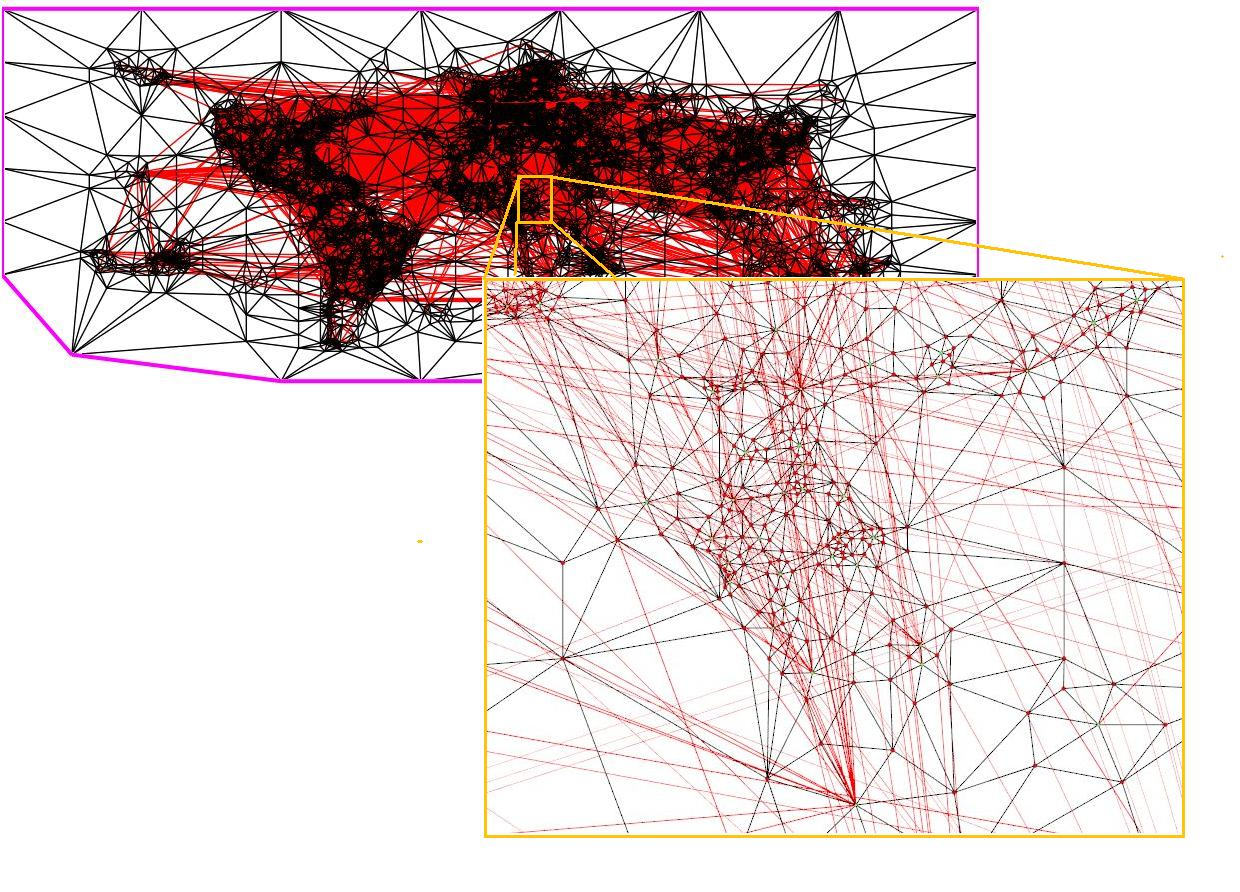
\includegraphics[scale=0.17]{../rapport/img/problematic.jpg}
      \end{figure}
    \end{column}
  \end{columns}
} 
